\subsection{Image filtering}
Our last experiment consists in applying some filters to 18 images selected from our ImageNet subset, to see how
these changes can affect the image colorization output.
We appplied the following filters:
\begin{itemize}
	\item a blurring filter with three different intensities, corresponding to three different kernel sizes: 3, 7, 11;
	\item a cartoonizing filter;
	\item increasing and decreasing the image contrast;
	\item increasing and decreasing the image luminance.
\end{itemize}

We noticed that, in general, a blurred image is harder to colorize, and the more blurred the image is, the worse
the final colorization in all of the models.
On the contrary, images with a higher contrast and images with a higher luminance get a better colorization
in all the models, with just a few exceptions depending on the specific image.

In Figure \ref{fig:filter} we report an example of the outcome of the ChromaGAN model on the filtered images. We
can clearly see that the cartoonized image is the one with the less realistic colors: it looks like the model
didn't recognize the grass. This is probably due to the fact that the models we used are not trained on
cartoonized images. Another badly colored image, is the blurred one: here the dogs have some wired pink/orange
spots on their fur.

\begin{figure*}[t]
	\centering
	\captionsetup[subfigure]{labelformat=empty}
		\begin{subfigure}[b]{0.1\textwidth}
		\centering
		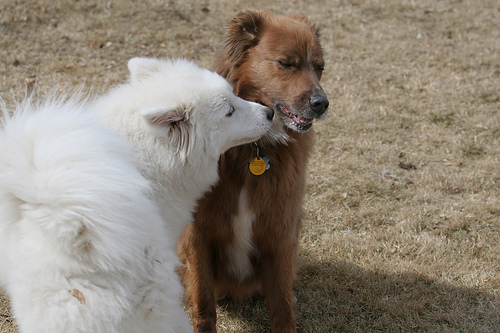
\includegraphics[width=2.4cm]{orig - filter.jpeg}
		\caption{Original}
		\end{subfigure}
		\hfill
		\begin{subfigure}[b]{0.1\textwidth}
			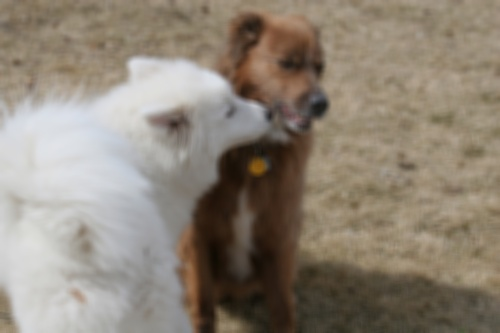
\includegraphics[width=2.4cm]{orig - filter - blur.jpeg}
			\caption{Blurred}
		\end{subfigure}
		\hfill
		\begin{subfigure}[b]{0.1\textwidth}
			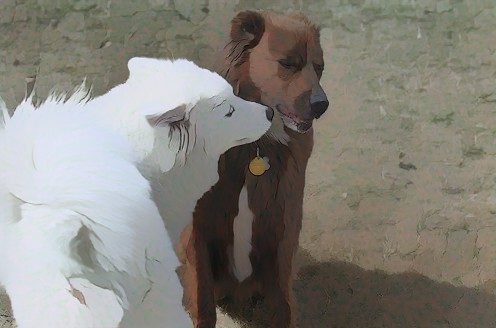
\includegraphics[width=2.4cm]{orig - filter - cartoon.jpeg}
			\caption{Cartoon}
		\end{subfigure}
		\hfill
		\begin{subfigure}[b]{0.1\textwidth}
			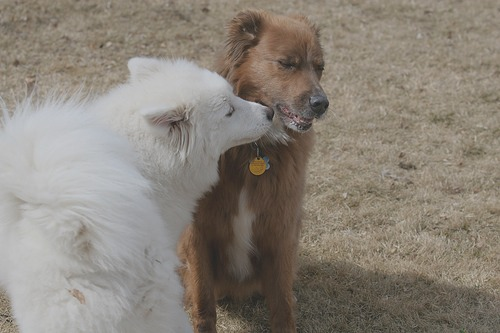
\includegraphics[width=2.4cm]{orig - filter - man contr (2).jpg}
			\caption{Low contrast}
		\end{subfigure}
		\hfill
		\begin{subfigure}[b]{0.1\textwidth}
			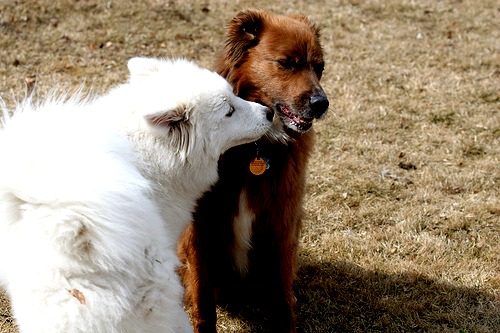
\includegraphics[width=2.4cm]{orig - filter - man contr (1).jpg}
			\caption{High contrast}
		\end{subfigure}
		\hfill
		\begin{subfigure}[b]{0.1\textwidth}
			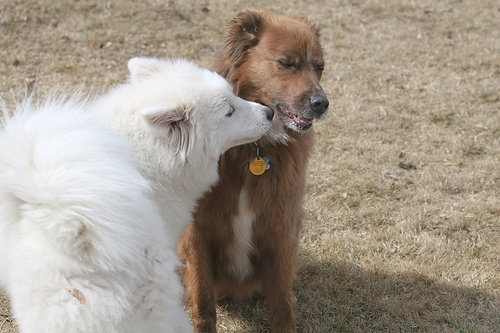
\includegraphics[width=2.4cm]{orig - filter - lumin (1).jpeg}
			\caption{Brighter}
		\end{subfigure}
		\hfill
		\begin{subfigure}[b]{0.1\textwidth}
			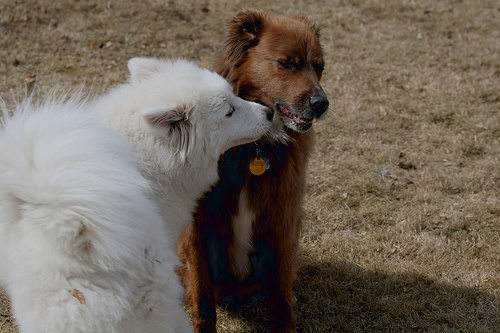
\includegraphics[width=2.4cm]{orig - filter - lumin (2).jpeg}
			\caption{Darker}
		\end{subfigure}
	
				\begin{subfigure}[b]{0.1\textwidth}
			\centering
			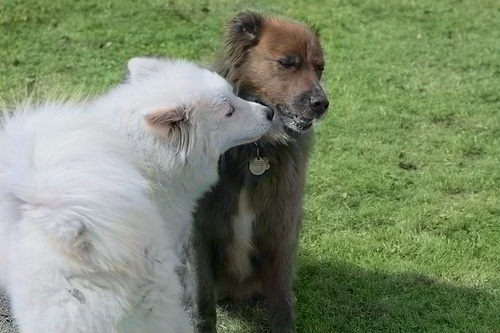
\includegraphics[width=2.4cm]{c - filter.jpeg}

		\end{subfigure}
		\hfill
		\begin{subfigure}[b]{0.1\textwidth}
			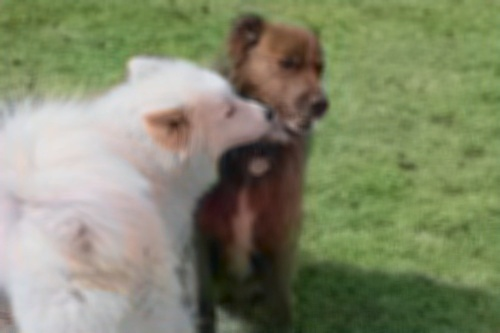
\includegraphics[width=2.4cm]{c - filter - blurr.jpeg}
		\end{subfigure}
		\hfill
		\begin{subfigure}[b]{0.1\textwidth}
			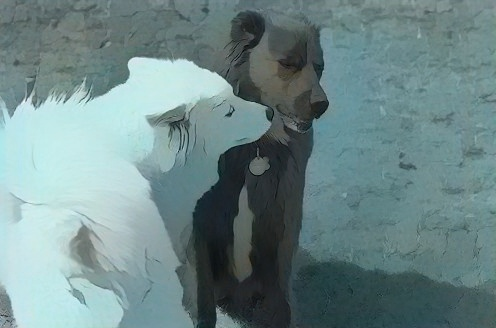
\includegraphics[width=2.4cm]{c - filter - cartoon.jpeg}
		
		\end{subfigure}
		\hfill
		\begin{subfigure}[b]{0.1\textwidth}
			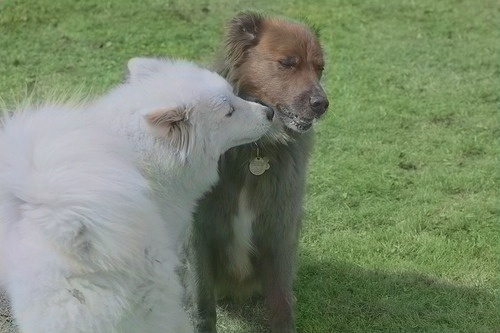
\includegraphics[width=2.4cm]{c - filter - man contr (1).jpg}
	
		\end{subfigure}
		\hfill
		\begin{subfigure}[b]{0.1\textwidth}
			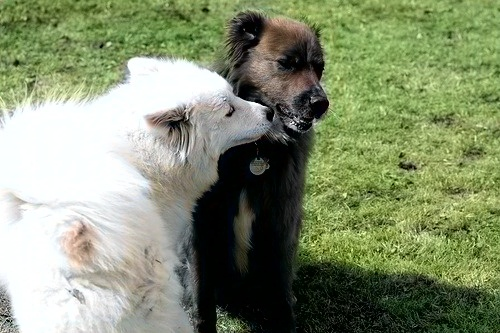
\includegraphics[width=2.4cm]{c - filter - man contr (2).jpg}
	
		\end{subfigure}
		\hfill
		\begin{subfigure}[b]{0.1\textwidth}
			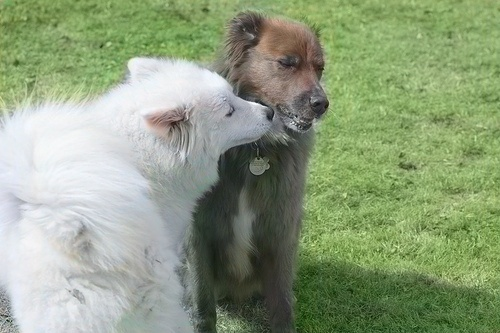
\includegraphics[width=2.4cm]{c - filter - lumin (1).jpeg}
	
		\end{subfigure}
		\hfill
		\begin{subfigure}[b]{0.1\textwidth}
			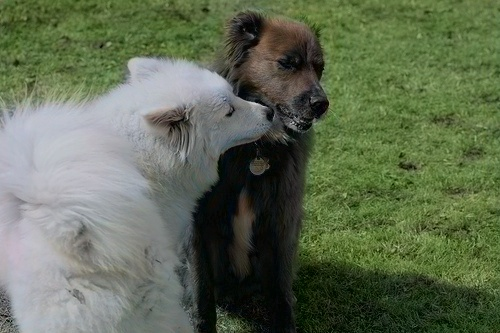
\includegraphics[width=2.4cm]{c - filter - lumin (2).jpeg}
	
		\end{subfigure}
	\caption{{\small ChromaGAN colorization (second row) on some filtered images (first row).}}
	\label{fig:filter}
\end{figure*}